% --- A R C H I T E K T U R S T I L E ---

Wie in Abschnitt \ref{Softwarearchitektur} beschrieben, umfasst die Softwarearchitektur sowohl die Struktur eines Systems als auch die einzelnen Details seiner Umsetzung. Die Anforderungen eines Softwaresystems variieren je nach Art der Anwendung, weshalb unterschiedliche Ansätze erforderlich sind.

Im Laufe der Zeit haben sich bestimmte \glqq{Muster}\grqq\ etabliert, die als Architekturstile bezeichnet werden. 
Benannt werden diese nach bestimmten architektonischen Eigenschaften, die Aufschluss über die Topologie oder potenzielle Herausforderungen geben.

Die Wahl eines geeigneten Architekturstils ist von entscheidender Bedeutung, da sie die grundlegende Struktur des Systems festlegt und den Entwickler/innen als Leitfaden dient. Zudem wird vermieden, dass ein \textbf{\glqq{Big Ball of Mud\footnote{Anti-Pattern, bei dem keine erkennbare Softwarearchitektur existiert}}\grqq}\ entsteht. 

Für eine fundierte Entscheidung wird die Anforderungsanalyse \ref{Projektbezug - Anforderungsanalyse} herangezogen, die festlegt, welche Aspekte besonders relevant sind. 

Ein paar gängige Beispiele:
\begin{itemize}
    \item Monolithische Architektur
    \item Serviceorientierte Architektur (SOA)
    \item Eventbasierte Architektur
    \item Serverlose Architektur
    \item Microservices-Architektur
\end{itemize}

Um den Fokus auf cloudbasierte Systeme zu richten, wird im Anschluss eine Auswahl relevanter Architekturstile beschrieben, die in modernen Cloud-Umgebungen besonders häufig Anwendung finden. 
\cite[S. 125-126]{EA:Book02} \cite{EA:Web60}


\clearpage


    % --- M I C R O S E R V I C E   A R C H I T E K T U R ---

    \subsection{Microservices-Architektur} \label{Microservices-Architektur}

    Die nach Fowler und Lewis benannte \glqq{Microservices-Architektur}\grqq\ ist einer der am häufigsten eingesetzten Architekturstile der heutigen Zeit. Besonders in den letzten Jahren hat dieser Architekturstil stark an Bedeutung gewonnen.

    Dabei wird nicht eine große Applikation entwickelt, die als eine Einheit bereitgestellt werden kann, sondern mehrere voneinander unabhängige Services, die miteinander interagieren und so ein System bilden. Es handelt sich um eine \textbf{verteilte Architektur}.
    Die Unterteilung in die einzelnen Komponenten erfolgt anhand des \textbf{Domain-Driven-Designs (DDD)}.
    \cite[S. 251-253]{EA:Book02}

    Ziel ist es, die grundlegenden Komponenten des Systems eigenständig zu betreiben, sodass im Falle eines Fehlers nur ein Dienst ausfällt und nicht das gesamte System. 
    \cite{EA:Web61}

        % --- A U F B A U ---
    
        \subsubsection{Aufbau}
    
        In Abbildung \ref{fig:microservices-topology} wird dargestellt, wie der allgemeine Aufbau einer Microservices-Architektur aussieht:
    
        \begin{figure}[H]
            \centering
            
\includegraphics[width=0.45\linewidth]{images/EA/microservices-topology.png}
            \caption{Microservices Topologie \\ \cite[S. 252]{EA:Book02}}
            \label{fig:microservices-topology}
        \end{figure}

        Grundsätzlich gibt es eine zentrale API-Schnittstelle, die die Anfragen der Clients an die entsprechenden Microservices weiterleitet.
        Bestehen Abhängigkeiten zwischen den Diensten, erfolgt die Kommunikation ebenfalls über die gemeinsame Schnittstelle.
        \cite{EA:Web61}

        Eine dedizierte Datenbank pro Service soll dabei für \textbf{Fehlertoleranz} sorgen, sodass, wie vorhin bereits erwähnt, nur die vom Fehler betroffenen Teile des Systems ausfallen, während andere Dienste und Daten weiterhin verfügbar bleiben.
        \cite[S. 268]{EA:Book02}

        Da es sich hierbei um einen cloudnativen Ansatz handelt, ist es üblich, moderne Methoden wie \textbf{DevOps} (siehe Abschnitt \ref{DevOps}) zu verwenden, um Software einfach und schnell zu entwickeln und in der Cloud bereitzustellen (siehe Unterkapitel \ref{Cloud Computing}). 
        Um dies zu ermöglichen, ist es oft notwendig, die Organisation so umzustrukturieren, dass sie in mehrere kleine Teams unterteilt wird, die für unterschiedliche Dienste verantwortlich sind. In der Theorie bietet dies den Vorteil, dass durch die unabhängigen Dienste weniger oder gar keine Konflikte mehr auftreten und die Auslieferung somit schneller erfolgen kann.
        \cite{EA:Web62}

        % --- V O R -   U N D   N A C H T E I L E ---

        \subsubsection{Vor- und Nachteile}

        Die Microservices-Architektur bietet dabei einige Vor- und Nachteile, die tabellarisch in \ref{tab:microservices-pros-and-cons} dargestellt werden. Bei einer gut durchdachten Umsetzung können einige der aufgelisteten Nachteile vermieden werden. \\
        \cite[S. 253, 268-269]{EA:Book02} \cite{EA:Web62} \\

        \begin{table}[H]
            \centering
            \begin{tabular}{|p{7.5cm}|p{7.5cm}|}
                \hline
                \cellcolor{green!40} \textbf{Vorteile} & \cellcolor{red!40} \textbf{Nachteile} \\ \hline
                 + Unterstützung agiler Vorgehensweisen & - Netzwerkbedingte Performanceverluste \\
                 + Hohe Fehlertoleranz & - Komplexer Aufbau \\ 
                 + Flexible Skalierung & - Erschwertes Testen \& Debuggen \\
                 + Einfache Wartung \& Erweiterbarkeit & - Erhöhter Ressourcenbedarf \\
                 \hline
            \end{tabular}
            \caption{Vor- und Nachteile der Microservices-Architektur}
            \label{tab:microservices-pros-and-cons}
        \end{table}


        % --- E I N S A T Z G E B I E T E ---

        \subsubsection{Einsatzgebiete}

        Unternehmen, die eine Vielzahl unterschiedlicher Dienste über das Internet bereitstellen, profitieren von den Vorteilen der Microservices-Architektur. Diese hat nicht nur einen positiven Einfluss auf die Softwareentwicklung, sondern optimiert auch die Nutzererfahrung. \\
        Denn durch die flexible Skalierung einzelner Applikationen lassen sich Engpässe durch gezieltes Hinzufügen oder Entfernen von Ressourcen effektiv vermeiden.
        \cite{EA:Web62}

        Folgende Beispiele verdeutlichen die Relevanz der Microservices-Architektur:
        \begin{itemize}
            \item \textbf{Social-Media-Plattformen}
            \begin{itemize}[label=$\circ$]
                \item z.B. Instagram, Facebook, X, usw.
            \end{itemize}

            \item \textbf{Video-Streaming-Dienste} 
            \begin{itemize}[label=$\circ$]
                \item z.B. Netflix, Amazon Prime, usw.
            \end{itemize}
            
            \item \textbf{E-Commerce-Webseiten}
            \begin{itemize}[label=$\circ$]
                \item z.B. eBay, Amazon, usw.
            \end{itemize}
        \end{itemize}


    % --- E V E N T G E S T E U E R T E   A R C H I T E K T U R ---
    
    \subsection{Eventbasierte Architektur} \label{Eventbasierte Architektur}

    Ein weiterer Architekturstil, der oft im Zusammenhang mit der Microservices-Architektur eingesetzt wird, ist der \textbf{eventbasierte Architekturstil}. Ähnlich wie bei der Microservices-Architektur ist auch dies eine verteilte Architektur, bei der die \textbf{Kommunikation} zwischen den einzelnen Bestandteilen des Systems \textbf{asynchron\footnote{Senden/Empfangen von Daten ist zeitlich versetzt}} abläuft. \\
    \cite[S. 183]{EA:Book02}

    Wie bei anderen Architekturstilen gibt es verschiedene Möglichkeiten zur Umsetzung. In diesem Fall unterscheidet man zwischen \textbf{zwei Mustern}, die zur Realisierung einer eventbasierten Architektur genutzt werden:
    \begin{itemize}
        \item \textbf{Publisher \& Subscriber}
        \begin{itemize}[label=$\circ$]
            \item Subscriber erhalten Benachrichtigungen von den abonnierten Kanälen und reagieren darauf.  
        \end{itemize}
        
        \item \textbf{Event Streaming}
        \begin{itemize}[label=$\circ$]
            \item Subscriber können den gesamten Stream lesen
            \item Nur die für den Subscriber relevanten Informationen werden verarbeitet
        \end{itemize}
    \end{itemize}

    \cite{EA:Web63}


         % --- A U F B A U ---
    
        \subsubsection{Aufbau}

        Abbildung \ref{fig:event-driven-architecture-topology} stellt dabei eine Form der eventgesteuerten Architektur dar.

        \begin{figure}[H]
            \centering
            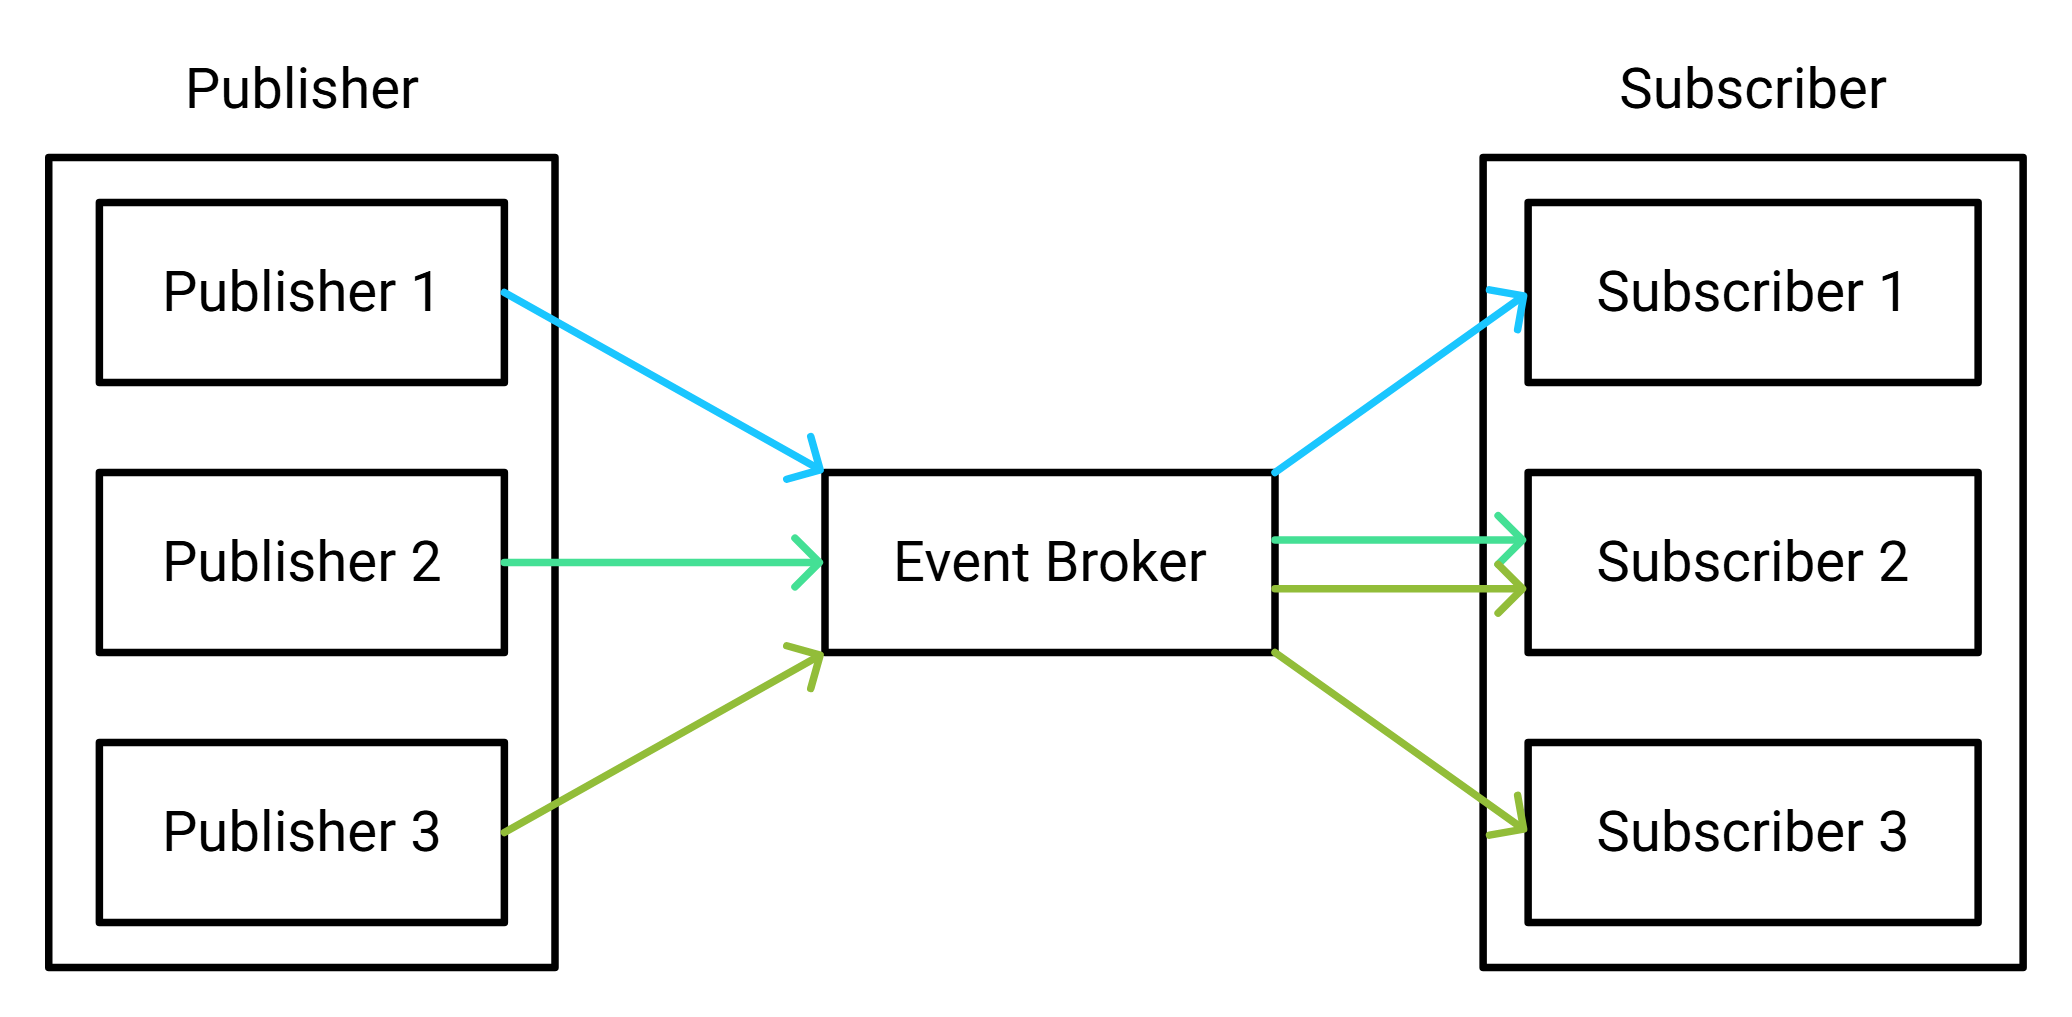
\includegraphics[width=0.9\linewidth]{images/EA/even-driven-architecture.png}
            \caption{Eventbasierte Architektur - Publisher/Subscriber \\ \cite{EA:Img02}}
            \label{fig:event-driven-architecture-topology}
        \end{figure}

        Das Publisher/Subscriber-Muster besteht aus folgenden Bestandteilen:
        \begin{itemize}
            \item \textbf{Publisher}
            \begin{itemize}[label=$\circ$]
                \item Lösen Ereignisse aus und senden diese an den Event Broker
                \item z.B. Bedienung einer Benutzeroberfläche 
            \end{itemize}
            
            \item \textbf{Subscriber}
            \begin{itemize}[label=$\circ$]
                \item Konsumieren und verarbeiten Ereignisse
                \item Empfangen Ereignisse abonnierter Event Channels des Brokers
            \end{itemize}
            
            \item \textbf{Broker}
            \begin{itemize}[label=$\circ$]
                \item Kümmert sich um die richtige Weiterleitung der Ereignisse
            \end{itemize}
        \end{itemize}

        \cite{EA:Web63}
        
        \clearpage
        
        % --- V O R -   U N D   N A C H T E I L E ---
    
        \subsubsection{Vor- und Nachteile}

        Die eventbasierte Architektur bietet einige Vor- und Nachteile:
    
        \begin{table}[H]
            \centering
            \begin{tabular}{|p{7.5cm}|p{7.5cm}|}
                \hline
                \cellcolor{green!40} \textbf{Vorteile} & \cellcolor{red!40} \textbf{Nachteile} \\ \hline
                 + Hohe Fehlertoleranz & - Erschwertes Testen \& Debuggen \\
                 + Hohe Performance & - Risiko von Datenverlusten \\ 
                 + Hohe Skalierbarkeit & - Komplexer Ablauf \& Implementierung \\
                 + Einfache Erweiterbarkeit & - Schwierige Fehlerbehandlung \\
                 + Echtzeitunterstützung & ~ \\
                \hline
            \end{tabular}
            \caption{Vor- und Nachteile der eventbasierten Architektur}
            \label{tab:event-driven-architecture-pros-and-cons}
        \end{table}

        Da dieser Architekturstil ebenfalls auf den Konzepten verteilter Systeme basiert, bietet er ähnliche Vorteile wie die Microservices-Architektur. Zudem eignet sich die ereignisgesteuerte Architektur für Echtzeit-Anwendungen, da sofort auf eintretende Ereignisse reagiert werden kann.
        
        Allerdings bringt die asynchrone Kommunikation einige Herausforderungen mit sich. Dazu zählt insbesondere die \textbf{Koordination der einzelnen Events}, sodass deren Reihenfolge erhalten bleibt und ein kontrollierter Ablauf gewährleistet wird. Da Ereignisse dynamisch eintreten, ist es oft schwierig, den genauen Ablauf nachzuvollziehen und mögliche Fehlerquellen zu identifizieren. \\
        \cite[S. 183, S. 205, S. 211-213]{EA:Book02}
    
        % --- E I N S A T Z G E B I E T E ---
    
        \subsubsection{Einsatzgebiete}

        Der eventgesteuerte-Architekturstil hat zahlreiche Anwendungsfälle in den unterschiedlichsten Bereichen.
        Dazu gehören:
        \begin{itemize}
            \item \textbf{Finanzapplikationen}
            \begin{itemize}[label=$\circ$]
                \item z.B. Subscriber informieren, sobald sich der Kurs einer Aktie ändert
            \end{itemize}

            \item \textbf{Internet of Things (IoT)}
            \begin{itemize}[label=$\circ$]
                \item z.B. Überwachung von Sensordaten
            \end{itemize}

            \item \textbf{Software im Gesundheitswesen}
            \begin{itemize}[label=$\circ$]
                \item z.B. Automatische Aktualisierung von Patientendaten
            \end{itemize}
        \end{itemize}

        \cite{EA:Web64} \cite[S. 184]{EA:Book02}

    \clearpage


    % --- S E R V E R L E S S   A R C H I T E K T U R ---
    
    \subsection{Serverlose Architektur}

    Der letzte cloudnative Architekturstil, der im Zuge dieser Arbeit beschrieben wird, ist die \textbf{serverlose Architektur}. 
    Bei dieser Art von Architektur steht weniger der eigentliche Aufbau eines Systems im Vordergrund, sondern die Verwaltung der benötigten Ressourcen. Die serverlose Architektur wird häufig in Kombination mit der Microservices-Architektur (siehe \ref{Microservices-Architektur}) oder der ereignisgesteuerten Architektur (siehe \ref{Eventbasierte Architektur}) eingesetzt. 

    Ziel dieser Architektur ist es, den Fokus der Entwickler/innen auf das Schreiben des eigentlichen Codes zu lenken, ohne sich mit den Anforderungen der für den Betrieb notwendigen IT-Infrastruktur auseinandersetzen zu müssen. Stattdessen übernimmt ein entsprechender Cloud-Dienstanbieter diese Aufgabe, einschließlich der Bereitstellung und Skalierung der Applikationen. Dadurch muss ein Unternehmen \textbf{nur für die tatsächlich verwendeten Rechenressourcen bezahlen}.

    Wird eine bereitgestellte Applikation nicht verwendet, so werden auch keine Ressourcen benötigt. Das heißt, \textbf{Ressourcen werden dynamisch bereitgestellt}.

    Die serverlose Architektur lässt sich dabei in zwei Bereiche eingliedern:
    \begin{enumerate}
        \item \textbf{Backend-as-a-Service (BaaS)}
        \begin{itemize}[label=$\circ$]
            \item Integration von Drittanbieterdiensten und Applikationen möglich
            \item Kommunikation erfolgt über APIs
            \item Auslagerung bestimmter Funktionalitäten - z.B. Authentifizierung
        \end{itemize}
        
        \item \textbf{Function-as-a-Service (FaaS)}
        \begin{itemize}[label=$\circ$]
            \item Ereignisgesteuert
            \item Bereitgestellter Code wird nur bei Aufruf ausgeführt
        \end{itemize}
    \end{enumerate}

    Da es für diesen Architekturstil keine allgemein gültige Topologie gibt, sondern abhängig ist von der eingesetzten Technologie, wird auf die Darstellung des Aufbaus verzichtet. Stattdessen werden Technologien genannt, die für die Umsetzung einer serverlosen Architektur verwendet werden können:
    \begin{itemize}
        \item AWS Lambda
        \item Azure Functions
        \item Google Cloud Functions
    \end{itemize}
    \cite{EA:Web65}
    
    \clearpage

        % --- V O R -   U N D   N A C H T E I L E ---

        \subsubsection{Vor- und Nachteile}

        In Tabelle \ref{tab:serverless-architecture-pros-and-cons} werden die wichtigsten Vor- und Nachteile des serverlosen Architekturstils aufgelistet:
    
        \begin{table}[H]
            \centering
            \begin{tabular}{|p{7.5cm}|p{7.5cm}|}
                \hline
                \cellcolor{green!40} \textbf{Vorteile} & \cellcolor{red!40} \textbf{Nachteile} \\ \hline
                 + Kosteneinsparungen & - Neue Sicherheitsrisiken \\
                 + Erhöhte Produktivität & - Mögliche Einschränkungen \\ 
                 + Hohe Skalierbarkeit & - Erhöhte Latenz \\
                 + Integration von Drittanbietersoftware & - Weniger Kontrollmöglichkeiten \\
                \hline
            \end{tabular}
            \caption{Vor- und Nachteile der serverlosen Architektur}
            \label{tab:serverless-architecture-pros-and-cons}
        \end{table}
        \cite{EA:Web66}
    
         % --- E I N S A T Z G E B I E T E ---
    
        \subsubsection{Einsatzgebiete}

        Wie für die zuvor genannten Architekturstile, kann auch die serverlose Architektur in unzähligen Bereichen eingesetzt werden:
        \begin{itemize}
            \item Backend-Applikationen
            \item Spezielle Aufgaben, die in einem festgelegten Intervall ausgeführt werden
            \begin{itemize}[label=$\circ$]
                \item Berichte generieren
                \item Backup einer Datenbank erstellen
            \end{itemize}
            \item Webapplikationen mit schwer vorhersehbarer Nachfrage
        \end{itemize}
        \cite{EA:Web65}

    \clearpage


    % --- P R O J E K T B E Z U G ---
    
    \subsection{Projektbezug - Architekturstil} \label{Projektbezug - Architekturstil}

    Basierend auf der Anforderungsanalyse (siehe Abschnitt \ref{Projektbezug - Anforderungsanalyse}) wird eine geeignete Architektur für das Projekt ausgewählt. Die folgenden Punkte fassen die für das Projekt CGM MAXX LITE relevanten Anforderungen zusammen:
    \begin{itemize}
        \item \textbf{Funktionale Anforderungen:}
        \begin{itemize}[label=$\circ$]
            \item Patientensuche und Darstellung der zugehörigen Daten
            \item Hinterlegung von Bildern und Audiodateien in der Patientenakte
        \end{itemize}
        
        \item \textbf{Nicht-funktionale Anforderungen:}
        \begin{itemize}[label=$\circ$]
            \item Hohe Ausfallsicherheit
            \item Skalierbarkeit einzelner Komponenten
            \item Erweiterbarkeit für zukünftige Funktionalitäten
        \end{itemize}
    \end{itemize}

    Die funktionalen Anforderungen lassen sich dabei in zwei Bereiche unterteilen:
    \begin{enumerate}
        \item Verwaltung von Patientendaten
        \item Verwaltung von Dateien
    \end{enumerate}

    Unter Berücksichtigung der zuvor beschriebenen Architekturstile (siehe Unterkapitel \ref{Architekturstile}) eignet sich die \textbf{Microservices-Architektur} besonders gut. Zudem ermöglicht sie es, die Software in zwei Subdomänen zu unterteilen. Dadurch lassen sich die Kernfunktionalitäten der Software in zwei unabhängige Services auslagern, was die \textbf{Fehlertoleranz} und \textbf{Wartbarkeit} erhöht.

    Sowohl die ereignisgesteuerte Architektur als auch die Ansätze des serverlosen Computings hätten sich ebenfalls für die Umsetzung von CGM MAXX LITE geeignet. Da der Fokus jedoch auf der Entwicklung der Benutzeroberfläche liegt und der Wunsch des Auftraggebers ist, die Software so zu gestalten, dass anstelle des von uns entwickelten Backends das Backend der Desktop-Applikation CGM MAXX angebunden werden kann, fiel die Entscheidung auf eine einfache Microservices-Architektur.

    Zur Implementierung wird das Java-Framework \textbf{Spring Boot} in Kombination mit der \textbf{Spring Cloud} Library eingesetzt.
    Diese Entscheidung basiert sowohl auf den umfangreichen Funktionalitäten der Technologie als auch auf den Erfahrungen der Projektteammitglieder.

    Im Folgenden wird die genaue Umsetzung von CGM MAXX LITE näher erläutert.

    \begin{figure}[H]
        \centering
        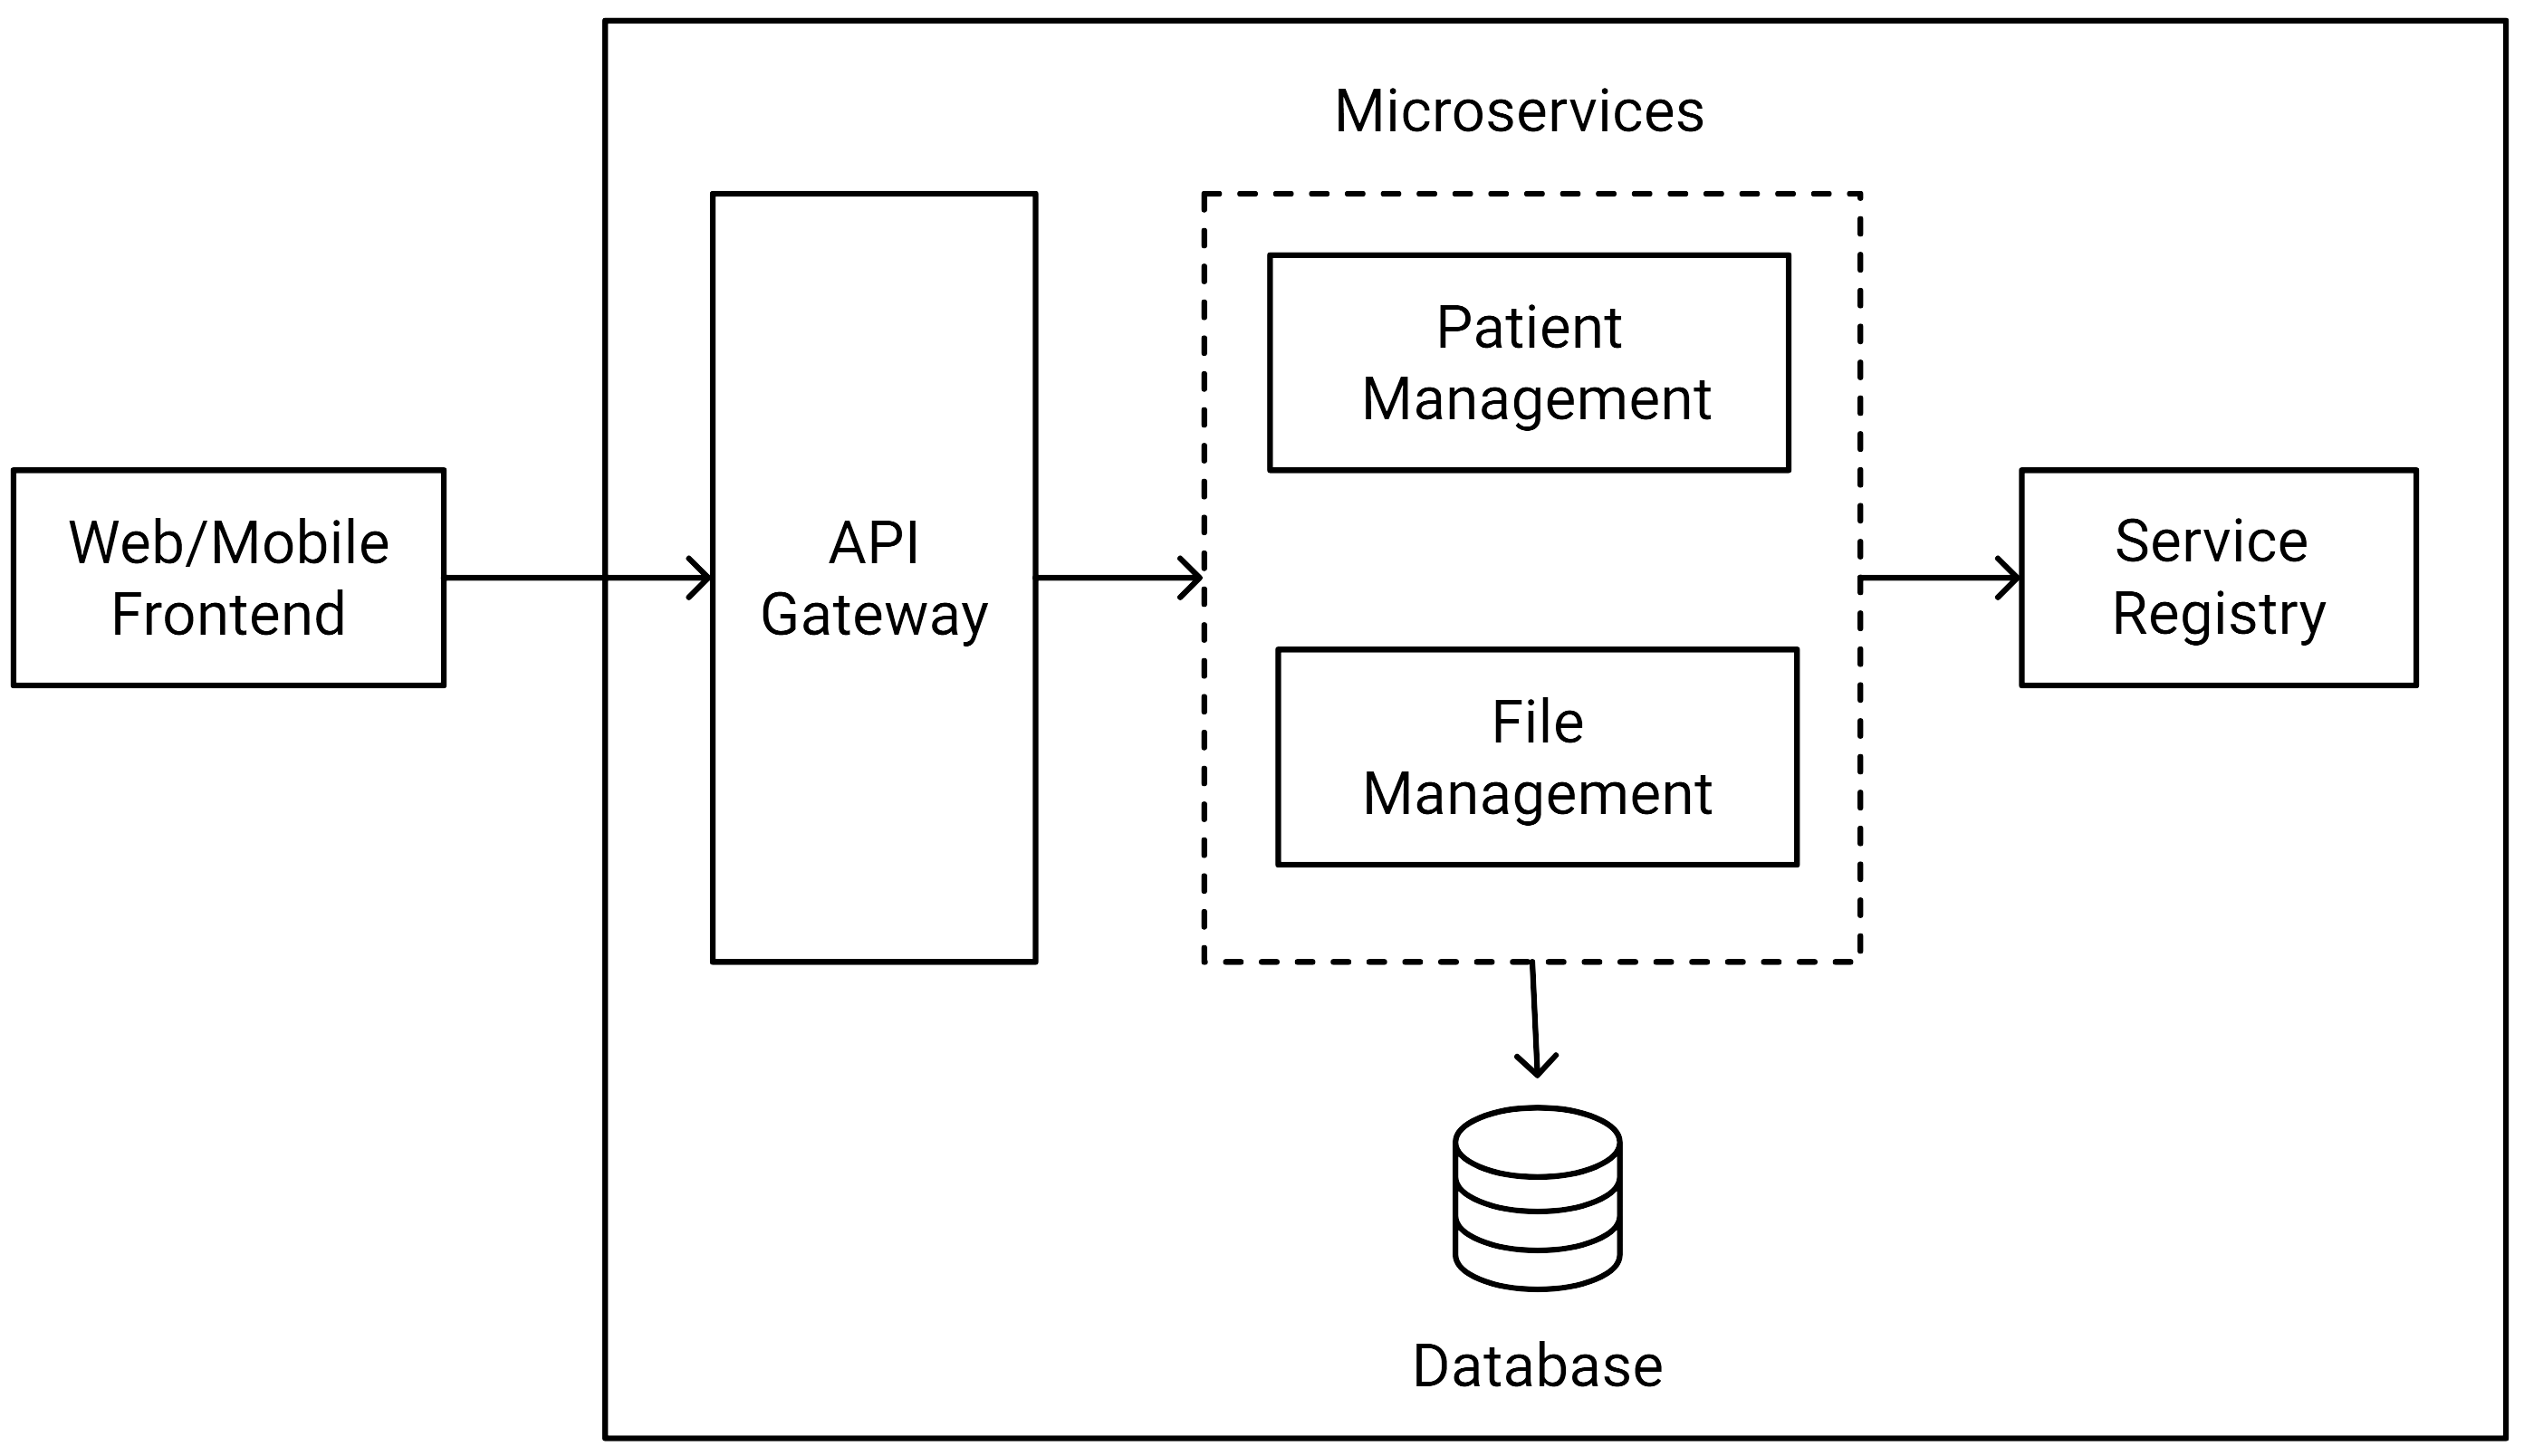
\includegraphics[width=0.95\linewidth]{images/EA/microservice-architecture.png}
        \caption{Microservice Architektur - CGM MAXX LITE}
        \label{fig:cgm-maxx-lite-microservices-architecture}
    \end{figure}

    Abbildung \ref{fig:cgm-maxx-lite-microservices-architecture} zeigt den Aufbau von CGM MAXX LITE mithilfe von Spring Boot. \\
    Die Software besteht aus folgenden Komponenten:
    \begin{itemize}
        \item \textbf{Web/Mobile Frontend}
        \begin{itemize}[label=$\circ$]
            \item Schnittstelle für Benutzerinteraktionen
            \item Kommuniziert mit der API, um Daten zu empfangen und zu senden
        \end{itemize}
        
        \item \textbf{API-Gateway}
        \begin{itemize}[label=$\circ$]
            \item Leitet eingehende Requests an die zuständigen Microservices weiter
        \end{itemize}
        
        \item \textbf{Microservices}
        \begin{itemize}[label=$\circ$]
            \item Patient Management \& File Management
        \end{itemize}

        \item \textbf{PostgreSQL-Datenbank}
        \begin{itemize}[label=$\circ$]
            \item Speichert alle Patientendaten sowie zugehörige Dateien
        \end{itemize}
        
        \item \textbf{Netflix Eureka Service Registry}
        \begin{itemize}[label=$\circ$]
            \item Registriert alle zum System gehörigen Microservices
            \item Ermöglicht die Kommunikation zwischen diesen
        \end{itemize}
    \end{itemize}

    In der Theorie wird für jedes Microservice eine eigene Datenbank erstellt, um eine höhere Ausfallsicherheit zu gewährleisten. 
    Aufgrund begrenzter Ressourcen, insbesondere in Bezug auf die Hardwareleistung und den zeitlich begrenzten Projektrahmen, wird eine zentrale Datenbank verwendet.

    Nun folgt eine genauere Beschreibung des Backends. Nicht nur die Microservices, sondern auch das API-Gateway
    müssen vom Service Registry registriert werden. Dies ist notwendig, um die vom Frontend kommenden Anfragen korrekt weiterzuleiten und die Kommunikation zwischen den Microservices zu ermöglichen. \lil{lst:service-registry-config} zeigt die Konfigurationsdatei der Service Registry Anwendung. \\
    
    \lstinputlisting[
        caption=\texttt{application.properties} - Service Registry,
        label=lst:service-registry-config,
    ]{sources/EA/application.properties}

    Grundsätzlich läuft die Service Registry auf dem Port 8761. Wird dieser Port freigegeben, kann über den Browser ein Dashboard aufgerufen werden, das alle registrierten Services auflistet. Zudem ist sie so konfiguriert, dass sie sich nicht selbst registriert. Bei den Microservices müssen die Werte \textbf{register-with-eureka} und \textbf{fetch-registry} auf \textbf{true} gesetzt werden. \lil{lst:file-service-config} zeigt einen Ausschnitt der Konfiguration des File Service: \\

    \lstinputlisting[
        caption=\texttt{application-docker.properties},
        label=lst:file-service-config,
    ]{sources/EA/application-docker.properties}

    Zusätzlich wird definiert, über welche URL die Service Registry erreicht werden kann. Da der File Service vor dem Hochladen einer Datei überprüfen muss, ob ein Patient mit der angegebenen ID existiert, benötigt dieser Zugriff auf den Patient Service.
    In Zeile 10 wird die URL des Patient Services definiert. Diese muss mit der im API-Gateway festgelegten URL (siehe \lil{lst:api-gateway}) übereinstimmen.

    Grundsätzlich ist kein API-Gateway notwendig. Allerdings erleichtert eine zentrale Schnittstelle die Verwaltung, da nur ein einziger Port nach außen hin freigegeben werden muss. 

    Im Folgenden werden jeweils ein REST-Controller des Patient Services und des File Services gezeigt, um einen Überblick über die verschiedenen Endpunkte zu geben. \\

    \lstinputlisting[
        caption=\texttt{PatientController.java},
        label=lst:patient-controller,
        firstline=16
    ]{sources/EA/PatientController.java}

    \lstinputlisting[
        caption=\texttt{FileInfoController.java},
        label=lst:file-info-controller,
        firstline=13
    ]{sources/EA/FileInfoController.java}

    Damit soll gezeigt werden, dass die Endpunkte verschiedener Anwendungen, die auf unterschiedlichen Ports betrieben werden, mithilfe eines API-Gateways über eine einzige Schnittstelle erreicht werden können.

    \clearpage

    Eine kurze Zusammenfassung der wichtigsten Endpoints:
    \begin{itemize}
        \item \textbf{PatientController} (siehe \lil{lst:patient-controller}) - Patient Management (Port 8081)
        \begin{itemize}[label=$\circ$]
            \item findPatients
            \item findById
        \end{itemize}
        
        \item \textbf{FileInfoController} (siehe \lil{lst:file-info-controller}) - File Management (Port 8082)
        \begin{itemize}[label=$\circ$]
            \item findFileById
            \item findFilesByPatientIdAndType
        \end{itemize}
    \end{itemize}

    Wird nun das Frontend gestartet, so werden verschiedene HTTP-Requests an das API-Gateway gesendet. 
    Werden die Dev-Tools in einem beliebigen Browser geöffnet und der Netzwerk-Tab ausgewählt, so kann überprüft werden, ob die Requests an den richtigen Microservice weitergeleitet werden.

    Klickt ein Arzt oder eine Ärztin auf eine bestimmte Person in der Patientenliste, so wird eine Detailansicht mit genaueren Informationen geöffnet. Dabei wird ein HTTP-Request an das Backend gesendet, um weitere Daten zu laden. 

    \begin{figure}[H]
        \centering
        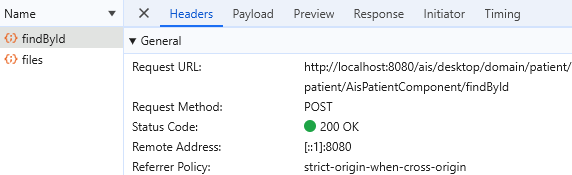
\includegraphics[width=1\linewidth]{images/EA/patient-management-http-request.png}
        \caption{HTTP-Request an den Patient Service}
        \label{fig:patient-management-http-request}
    \end{figure}

    Abbildung \ref{fig:patient-management-http-request} zeigt den HTTP-Request an den Patient Service, der korrekt über das API-Gateway und den Port 8080 weitergeleitet wird.

    Neben den Stammdaten werden auch Fotos und Audiodateien abgerufen, wobei der Request an den File Service weitergeleitet wird, wie in Abbildung \ref{fig:file-management-http-request} dargestellt.

    \begin{figure}[H]
        \centering
        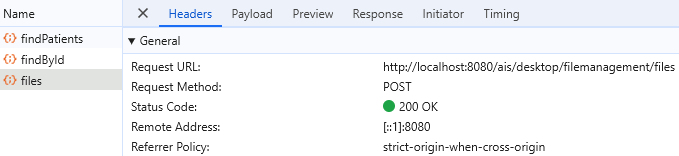
\includegraphics[width=1\linewidth]{images/EA/file-management-http-request.png}
        \caption{HTTP-Request an den File Service}
        \label{fig:file-management-http-request}
    \end{figure}

    Durch diese Architektur kann CGM MAXX LITE flexibel skaliert und durch die Entkopplung in mehrere Komponenten problemlos erweitert werden, was die Weiterentwicklung für die CGM Arztsysteme GmbH vereinfacht. 
    Im nächsten Kapitel wird das Thema Cloud Computing näher untersucht, um eine geeignete Lösung für den Betrieb der Software zu finden und die Unterschiede verschiedener Cloud-Modelle zu verdeutlichen. 
    